\part{Rasterizer}


\section{Introduction}
Rasterization is an object order method. We have a list of objects in our scene and draw one after another. This is the opposite of an image order rendering technique, like raytracing, where each pixel is traversed. This is why raytracing can be slower than rasterization; -testing each pixel and, for each pixel, testing every object. This pipeline can require more computation than a rasterization pipeline, which is iterating over every object once and coloring the pixels the object occupies.

Raytracing can be accelerated by spatial sorting, like bounding volume hierarchies, but so can rasterization. Frustrum- and occlusion-culling are just two examples.

The most basic job of a rasterizer is to draw triangles using pixels on a raster display. A popular method is scanline rendering, because of cache locality and the way displays update their image a scanline at a time.

\begin{figure}[H]
  \centering
  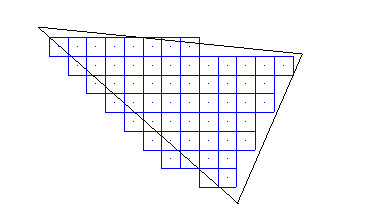
\includegraphics{Media/raster_scanline.png}
  \caption{Scanline rasterization of pixels}   
  \label{fig:Scanline rasterization of pixels}
\end{figure}


\section{Rasterization Pipelines}

Write something general about rasterization pipelines, to introduce the concept.


\subsection{Forward Rendering}

The rasterization and shading complexity of a forward rendering pipeline is

\begin{equation}\label{eq:FRP_complexity}
  \orderof(\sum {pixel_{rasterized + shaded}} \times \sum light)
\end{equation}

In a forward rendering pipeline (FRP), all surfaces are shaded immediately. As equation \eqref{eq:FRP_complexity} shows, this doesn't scale well as the number of lights go up.

\subsubsection{Multiple Lights}

There are different methods for dealing with multiple lights in an FRP. These different approaches all have their strengths and weaknesses.

\paragraph{Ubershader}

The Ubershader is a single-pass shader that handles any material and light combination or programatically create different shaders for all material- and light-type combinations. Creating an uber-shader becomes unwieldy as the types of lights and materials increase due to combinatorial explosion, each material-light pair will require custom code.

\paragraph{Multi-pass}

Another way of shading a surface with an arbitrary number lights is using a multi-pass technique. Each geometry is shaded with each light at a time. The framebuffer is set to blend fragments together, combining the effect of each light. Multi-pass rendering requires re-drawing the entire mesh for each light and requires transforming vertices and rasterizing each pass, making the scene quickly vertex and fillrate bound.

\subsection{Deferred Rendering}

The rasterization and shading complexity of a deferred rendering pipeline is
\begin{equation}\label{eq:DRP_complexity}
		\orderof(\sum {pixel_{rasterized}}) + \orderof(\sum {pixel_{GBuffer}} \times \sum {light})
\end{equation}

Deferred Rendering Deering1988 is a rasterization-based rendering technique in which the result of drawing the scene is divided and stored in intermediate buffers (called the G-Buffer) using multiple render targets (MRT).  The G-buffer, or Geometry-Buffer, is called so because it stores per pixel geometric properties like depth, normals and texture coordinates; - a caching of the geometry that the camera is viewing, for repeated use further down the rendering pipeline. The G-Buffer is input into a shading algorithm, usually as samplers, to produce the final result. This reduces the input of the scene to what is in the view space when performing shading, and specially reduce the cost of lighting. Lights are rendered in a second pass as geometric volumes, who's surface color is accumulated into a final render target using additive blending. In essence, this gives us a rendering pipeline which drives a single pass per light, as opposed to forward rendering's single pass with a complex shader or multi-pass techniques (typically single pass per mesh per light).

Historically, deferred rendering has had some limitations. Due to the nature of the G-Buffer, transparency couldn't be supported directly in the deferred pipeline. Instead, a forward renderer has commonly been used for handling transparent objects in the scene. Further, a deferred pipeline can't take advantage of Multisample anti-aliasing (MSAA) in hardware, forcing quite expensive anti-aliasing filters to be programmed into the pipeline. The amount of parameters one can pass to shader programs is also directly limited by the size of the G-Buffer, and the amount of render targets supported. This forces a deferred pipeline to be quite expensive, bandwidth and memory wise. Further, due to how a deferred pipeline accumulates the color of lights using additive blending, overlapping lights cause overhead.

On the positive side, a deferred rendering pipeline is greatly simplified and more general than a forward rendering pipeline. The scene is rendered with one shader program, filling the G-Buffer, and then the G-Buffer is handled in multiple passes by different shader programs, like the lighting pass, shadow pass, and so forth. These shader programs can also be simplified, as everything in the G-Buffer used for the shading, already is in screen-space. The cost for light calculation is greatly reduced compared to a forward renderer, since shading is only done in screen-space for geometry that is visible by the camera; -there is no wasted shading effort.

As equation \eqref{eq:DRP_complexity} shows, it scales much better with multiple lights than the forward rendering pipeline, in equation \eqref{eq:FRP_complexity}, does.

A deferred shading approach could lend well as a hybrid foundation of rasterization and raytracing, as the G-Buffer data could be generated by any method, as long as it is in screenspace, and could also be used as a first-ray lookup for a raytracer.

Over the years, multiple improvements to the deferred rendering approach has been applied in practise. Light pre-pass, tile-based deferred rendering and decoupled deferred rendering are listed among the most popular and more recent approaches.

\subsubsection{Light pre-pass}

Light pre-pass was first presented by Wolfgang Engel [Engel2008]. In this approach one would in a first pass render geometry information into a G-Buffer that is required for light-calculation, like depth, normals and specular power. In a second pass one would render the light geometry into a render-target using the G-Buffer for information about the scene. In a third pass, one would use normal forward-rendering, but use the light render target as sampler for the lighting, thus getting the reduced cost of lighting from a deferred rendering pipeline, while retaining much of the strengths and flexibility of a forward rendering pipeline. 

This forces three passes to render the scene, although each pass is cheaper than in a pure deferred pipeline, and consume less bandwidth and memory than the deferred pipeline. Using light pre-pass, one can even prevent usage of MRT. In essence, using this approach we end up with a pipeline which is single pass per mesh.

Looking at the limitations of light pre-pass, it still doesn't solve the problem with transparency in a deferred pipeline. Also, it is limited in variety of lighting due to the lighting buffer, and if sticking with a four-channel buffer for lights, both colored specular and more advanced shading models, like Oren-Nayar, isn't easy to achieve (although there are solutions to be found [BlindRenderer2011]). Further, the flexibility in the material properties of the third pass of the light pre-pass pipeline is illusive. One would think that the forward rendering nature of this pass would grant great flexibility in the property input to the shader program for each mesh, but what largely defines a material, is how its surface interacts with light. Thus, the limitations of the lighting buffer directly limits the flexibility of material properties.

On the positive side, we get hardware MSAA for the third geometry pass, even though the lighting buffer doesn't get this hardware anti-aliasing treatment.

\subsubsection{Tile-based Deferred Rendering}

A tile-based deferred rendering pipeline divides the screen space into tiles, the goal being to map which tiles each light intersects and thus greatly reduce the number of pixels to process for shading per light, and reduce the overhead of overlapping lights. In [Andersson2009], it's pointed out how the light-classification per screen-space tile is similar to how Compute Shaders can work with 2D thread-groups; - this is a case that should be convertible to other GPU compute APIs like OpenCL and Cuda. 

Using a computing API, the G-Buffer and depth is read only once, minimizing bandwidth, where a pure shader-based solution would have to multiple reads. All lighting is resolved with gpgpu before the shading result is finally written out to a buffer immediately available to the shader pipeline. Thus we don't need an intermediate light buffer, as with light pre-pass, and it scales much better with overlapping lights due to the fine-grained culling in tiles (eg. 16x16 tiles).